\chapter{Distributed Systems Through the Lens of Operating Systems}

\section{Introduction}

Operating systems manage resources, communication, concurrency, synchronization, memory, scheduling, and fault handling within a single machine. Distributed systems extend many of these concepts across multiple machines connected through a network.

Many distributed-system interview questions become easier when viewed through familiar operating-system concepts.

Examples:

\begin{itemize}
\item Processes become services
\item Threads become workers
\item Shared memory becomes distributed state
\item IPC becomes RPC
\item Mutexes become distributed locks
\item Scheduling becomes orchestration
\item Fault handling becomes distributed fault tolerance
\end{itemize}

\section{Why Distributed Systems Exist}

Single machines eventually hit limits.

Common limitations:

\begin{itemize}
\item CPU capacity
\item Memory capacity
\item Disk throughput
\item Network throughput
\item Availability requirements
\end{itemize}

Distributed systems address these limitations through:

\begin{itemize}
\item Horizontal scaling
\item Replication
\item Fault tolerance
\item Geographic distribution
\item Load sharing
\end{itemize}

Examples:

\begin{itemize}
\item Google Search
\item Amazon
\item Netflix
\item Uber
\item Meta
\end{itemize}

\section{OS Concepts vs Distributed Systems Concepts}

\begin{table}[H]
\centering
\begin{tabular}{ll}
\toprule
Operating Systems & Distributed Systems \\
\midrule
Process & Service \\
Thread & Worker \\
Memory & Distributed State \\
IPC & RPC \\
Mutex & Distributed Lock \\
Scheduler & Orchestrator \\
Shared Memory & Distributed Cache \\
File System & Distributed Storage \\
Kernel & Control Plane \\
Crash Recovery & Fault Tolerance \\
\bottomrule
\end{tabular}
\caption{OS Concepts vs Distributed Systems}
\end{table}

\section{Processes vs Services}

In operating systems:

\begin{itemize}
\item Process = executing program
\end{itemize}

In distributed systems:

\begin{itemize}
\item Service = independently deployable process
\end{itemize}

\begin{figure}[H]
\centering

\begin{tikzpicture}
\node[draw] (svc1) at (-4,0) {Auth Service};
\node[draw] (svc2) at (0,0) {User Service};
\node[draw] (svc3) at (4,0) {Payment Service};

\draw[<->] (svc1)--(svc2);
\draw[<->] (svc2)--(svc3);
\end{tikzpicture}
\caption{Services Communicating Across a Network}
\end{figure}

\section{Threads vs Workers}

Threads execute tasks within a process.

Distributed systems commonly use workers.

Examples:

\begin{itemize}
\item Kafka consumers
\item Celery workers
\item Background job processors
\item Spark executors
\end{itemize}

Worker pools resemble thread pools.

\section{Memory vs Distributed State}

Operating systems use local RAM.

Distributed systems store state across machines.

Examples:

\begin{itemize}
\item Redis clusters
\item Cassandra
\item DynamoDB
\item Distributed caches
\end{itemize}

\begin{figure}[H]
\centering
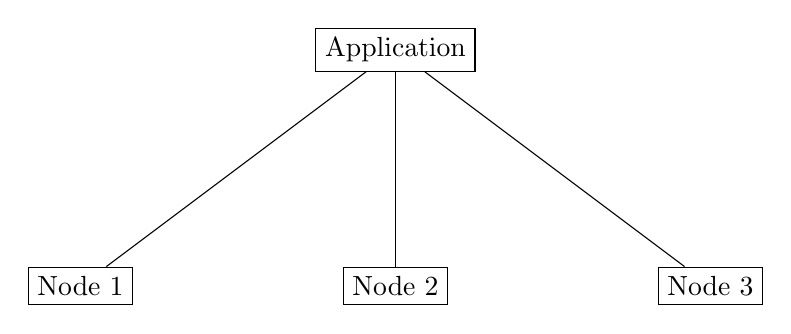
\begin{tikzpicture}
\node[draw] (app) at (0,3) {Application};

\node[draw] (n1) at (-4,0) {Node 1};
\node[draw] (n2) at (0,0) {Node 2};
\node[draw] (n3) at (4,0) {Node 3};

\draw (app)--(n1);
\draw (app)--(n2);
\draw (app)--(n3);
\end{tikzpicture}
\caption{Distributed State}
\end{figure}

\section{Local IPC vs Network Communication}

Operating systems provide IPC mechanisms:

\begin{itemize}
\item Pipes
\item Shared memory
\item Message queues
\item Sockets
\end{itemize}

Distributed systems use:

\begin{itemize}
\item HTTP
\item RPC
\item gRPC
\item Message brokers
\end{itemize}

Key difference:

\begin{itemize}
\item IPC assumes local machine reliability
\item Network communication assumes failures
\end{itemize}

\section{RPC Fundamentals}

Remote Procedure Call (RPC) allows one service to invoke functionality on another service as if calling a local function.

\subsection{RPC Workflow}

\begin{enumerate}
\item Client invokes function
\item Request serialized
\item Sent across network
\item Server executes request
\item Response serialized
\item Returned to client
\end{enumerate}

\begin{figure}[H]
\centering
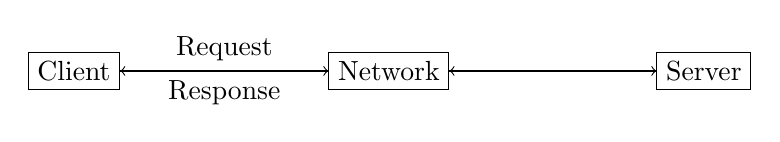
\begin{tikzpicture}
\node[draw] (client) at (-4,0) {Client};

\node[draw] (network) at (0,0) {Network};

\node[draw] (server) at (4,0) {Server};

\draw[->] (client)--node[above]{Request}(network);
\draw[->] (network)--(server);

\draw[<-] (client)--node[below]{Response}(network);
\draw[<-] (network)--(server);
\end{tikzpicture}
\caption{RPC Communication}
\end{figure}

\section{gRPC Overview}

gRPC is a high-performance RPC framework developed by \textbf{Google}.

Features:

\begin{itemize}
\item HTTP/2
\item Protocol Buffers
\item Streaming
\item Strong typing
\item Cross-language support
\end{itemize}

Advantages:

\begin{itemize}
\item Low latency
\item Compact messages
\item Efficient communication
\end{itemize}

\section{Distributed Locks}

A mutex protects resources on one machine.

Distributed locks protect resources across multiple machines.

Common implementations:

\begin{itemize}
\item Redis Redlock
\item ZooKeeper
\item etcd
\item Consul
\end{itemize}

Example:

\begin{enumerate}
\item Service A acquires lock
\item Service B waits
\item Service A releases lock
\item Service B proceeds
\end{enumerate}

\section{Consensus Basics}

Consensus is the process of multiple nodes agreeing on a value.

Requirements:

\begin{itemize}
\item Agreement
\item Validity
\item Termination
\end{itemize}

Applications:

\begin{itemize}
\item Metadata storage
\item Cluster management
\item Configuration systems
\item Leader election
\end{itemize}

Popular algorithms:

\begin{itemize}
\item Paxos
\item Raft
\item Zab
\end{itemize}

\section{Leader Election}

Distributed systems often elect one node as leader.

Responsibilities:

\begin{itemize}
\item Coordination
\item Metadata management
\item Decision making
\item Replication control
\end{itemize}

\begin{figure}[H]
\centering
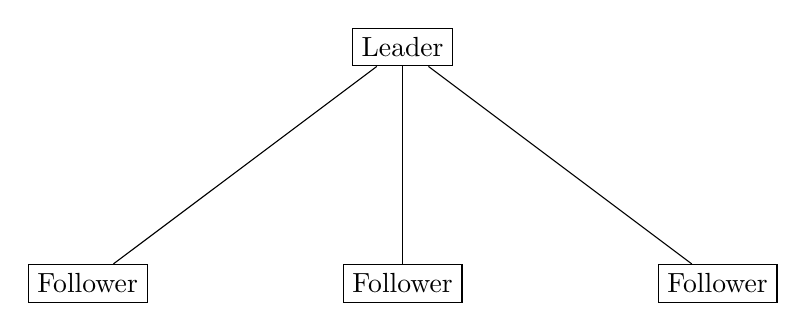
\begin{tikzpicture}
\node[draw] (leader) at (0,3) {Leader};

\node[draw] (n1) at (-4,0) {Follower};
\node[draw] (n2) at (0,0) {Follower};
\node[draw] (n3) at (4,0) {Follower};

\draw (leader)--(n1);
\draw (leader)--(n2);
\draw (leader)--(n3);
\end{tikzpicture}
\caption{Leader Election}
\end{figure}

\section{Clock Synchronization}

Distributed systems lack a perfectly shared clock.

Challenges:

\begin{itemize}
\item Network delay
\item Clock drift
\item Hardware differences
\end{itemize}

Common approaches:

\begin{itemize}
\item NTP
\item PTP
\item GPS clocks
\end{itemize}

\section{Logical Clocks}

Introduced by Lamport.

Purpose:

\begin{itemize}
\item Order events
\item Capture causality
\end{itemize}

Rule:

\[
C(a) < C(b)
\]

implies event \(a\) happened before event \(b\).

\section{Vector Clocks}

Vector clocks improve causal tracking.

Each node maintains a vector.

Example:

\[
[3,5,2]
\]

Advantages:

\begin{itemize}
\item Detect concurrent events
\item Capture causal relationships
\end{itemize}

\section{CAP Theorem}

A distributed system cannot simultaneously guarantee:

\begin{itemize}
\item Consistency
\item Availability
\item Partition Tolerance
\end{itemize}

During a partition:

\begin{itemize}
\item Choose Consistency
\item Or choose Availability
\end{itemize}

\begin{figure}[H]
\centering
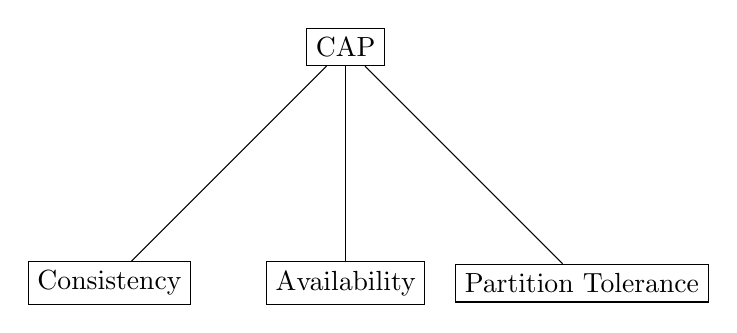
\begin{tikzpicture}
\node[draw] (cap) at (0,0) {CAP};

\node[draw] (c) at (-3,-3) {Consistency};
\node[draw] (a) at (0,-3) {Availability};
\node[draw] (p) at (3,-3) {Partition Tolerance};

\draw (cap)--(c);
\draw (cap)--(a);
\draw (cap)--(p);
\end{tikzpicture}
\caption{CAP Theorem}
\end{figure}

\section{Consistency Models}

\subsection{Strong Consistency}

Reads always return the latest write.

\subsection{Eventual Consistency}

Replicas eventually converge.

\subsection{Causal Consistency}

Causally related operations preserve order.

\subsection{Read-Your-Writes}

A client sees its own updates.

\subsection{Monotonic Reads}

Reads never move backward in time.

\section{Replication Basics}

Replication improves:

\begin{itemize}
\item Availability
\item Scalability
\item Fault tolerance
\end{itemize}

\subsection{Primary-Replica}

\begin{figure}[H]
\centering
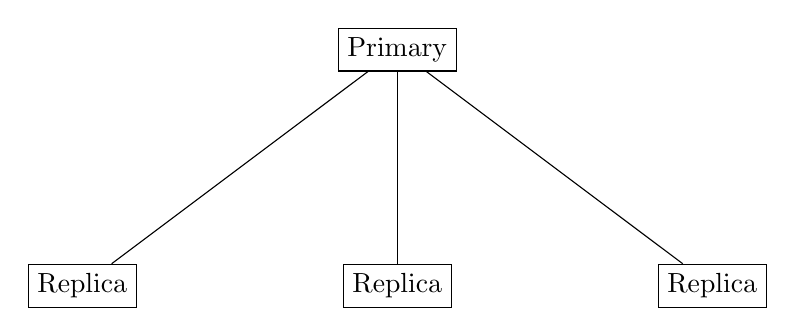
\begin{tikzpicture}
\node[draw] (primary) at (0,3) {Primary};

\node[draw] (r1) at (-4,0) {Replica};
\node[draw] (r2) at (0,0) {Replica};
\node[draw] (r3) at (4,0) {Replica};

\draw (primary)--(r1);
\draw (primary)--(r2);
\draw (primary)--(r3);
\end{tikzpicture}
\caption{Primary-Replica Replication}
\end{figure}

\subsection{Multi-Leader Replication}

Multiple leaders accept writes.

Advantages:

\begin{itemize}
\item Better geographic distribution
\end{itemize}

Challenges:

\begin{itemize}
\item Conflict resolution
\end{itemize}

\section{Fault Tolerance}

Distributed systems assume failures.

Common failures:

\begin{itemize}
\item Node failures
\item Disk failures
\item Network failures
\item Data-center failures
\end{itemize}

Strategies:

\begin{itemize}
\item Replication
\item Retries
\item Timeouts
\item Circuit breakers
\item Failover
\end{itemize}

\section{Distributed Transactions}

Transactions spanning multiple nodes.

Challenges:

\begin{itemize}
\item Partial failures
\item Network partitions
\item Consistency requirements
\end{itemize}

Common protocols:

\begin{itemize}
\item Two-Phase Commit (2PC)
\item Three-Phase Commit
\item Saga Pattern
\end{itemize}

\subsection{Two-Phase Commit}

\begin{enumerate}
\item Prepare Phase
\item Commit Phase
\end{enumerate}

Guarantees atomicity but may block.

\section{Modern Cloud Architectures}

Modern systems typically include:

\begin{itemize}
\item Microservices
\item Service mesh
\item Distributed databases
\item Message queues
\item Object storage
\item Containers
\item Kubernetes
\end{itemize}

\begin{figure}[H]
\centering
\begin{tikzpicture}
\node[draw] (users) at (0,6) {Users};

\node[draw] (gateway) at (0,4) {API Gateway};

\node[draw] (services) at (0,2) {Microservices};

\node[draw] (mq) at (-4,0) {Queue};
\node[draw] (db) at (0,0) {Database};
\node[draw] (cache) at (4,0) {Cache};

\draw (users)--(gateway);
\draw (gateway)--(services);

\draw (services)--(mq);
\draw (services)--(db);
\draw (services)--(cache);
\end{tikzpicture}
\caption{Modern Cloud Architecture}
\end{figure}

\section{Dedicated Interview Section: How OS Concepts Appear in Distributed Systems}

\begin{table}[H]
\centering
\begin{tabular}{ll}
\toprule
Operating System Concept & Distributed Equivalent \\
\midrule
Process & Service \\
Thread & Worker \\
Mutex & Distributed Lock \\
Shared Memory & Distributed Cache \\
IPC & RPC \\
Scheduler & Kubernetes Scheduler \\
Crash Recovery & Failover \\
File System & Distributed Storage \\
\bottomrule
\end{tabular}
\caption{Concept Mapping}
\end{table}

\section{Dedicated Interview Section: Distributed Lock Interview Questions}

\subsection*{Why are distributed locks needed?}

Multiple machines may attempt to modify the same resource.

\subsection*{How are distributed locks implemented?}

Commonly using:

\begin{itemize}
\item Redis
\item ZooKeeper
\item etcd
\end{itemize}

\subsection*{What can go wrong?}

\begin{itemize}
\item Lock expiration
\item Network partitions
\item Split-brain scenarios
\end{itemize}

\section{Dedicated Interview Section: Consistency Model Interview Questions}

\subsection*{What is strong consistency?}

Reads always return latest committed value.

\subsection*{What is eventual consistency?}

Replicas converge eventually.

\subsection*{Why choose eventual consistency?}

Improved availability and scalability.

\subsection*{Examples}

\begin{itemize}
\item Strong Consistency: etcd
\item Eventual Consistency: Dynamo-style systems
\end{itemize}

\section{Key Takeaways}

\begin{keytakeaways}
Distributed systems extend operating-system concepts across multiple machines. Processes become services, threads become workers, memory becomes distributed state, and IPC becomes RPC. Consensus algorithms, leader election, logical clocks, replication, fault tolerance, and consistency models are essential building blocks. CAP theorem explains trade-offs among consistency, availability, and partition tolerance. Understanding these mappings helps connect OS fundamentals with modern distributed-system design and interview problems.
\end{keytakeaways}

\section{Interview Questions with Answers}

\begin{enumerate}
\item Why do distributed systems exist?\\
To achieve scalability, availability, and fault tolerance.

\item What is the distributed equivalent of a process?\\
A service.

\item What is the distributed equivalent of a thread?\\
A worker.

\item What replaces IPC in distributed systems?\\
RPC and network communication.

\item What is RPC?\\
Remote Procedure Call.

\item What problem does gRPC solve?\\
Efficient service-to-service communication.

\item What transport does gRPC use?\\
HTTP/2.

\item What are Protocol Buffers?\\
Efficient binary serialization format.

\item What is a distributed lock?\\
A lock coordinating access across machines.

\item Why are distributed locks needed?\\
To prevent concurrent conflicting updates.

\item What is consensus?\\
Agreement among distributed nodes.

\item Name two consensus algorithms.\\
Raft and Paxos.

\item What is leader election?\\
Choosing one node to coordinate operations.

\item Why are clocks difficult in distributed systems?\\
They drift and cannot be perfectly synchronized.

\item What is a logical clock?\\
A mechanism for ordering events.

\item What is a vector clock?\\
A clock tracking causal relationships across nodes.

\item State the CAP theorem.\\
Cannot simultaneously guarantee consistency, availability, and partition tolerance.

\item What is strong consistency?\\
Reads always see the latest write.

\item What is eventual consistency?\\
Replicas eventually converge.

\item Why use replication?\\
Availability and fault tolerance.

\item What is a replica?\\
A copy of data on another node.

\item What is fault tolerance?\\
Ability to continue operating despite failures.

\item What is a distributed transaction?\\
A transaction spanning multiple nodes.

\item What is Two-Phase Commit?\\
A protocol for distributed atomic commits.

\item How do OS concepts help understand distributed systems?\\
Many distributed abstractions are extensions of OS abstractions.
\end{enumerate}

\section{MCQs with Answers}

\begin{enumerate}

\item Distributed systems primarily exist for:
\begin{enumerate}[label=(\alph*)]
\item Scaling
\item Availability
\item Fault Tolerance
\item All of the Above
\end{enumerate}
Answer: (d)

\item A service is analogous to a:
\begin{enumerate}[label=(\alph*)]
\item Process
\item Thread
\item Page
\item Cache
\end{enumerate}
Answer: (a)

\item RPC stands for:
\begin{enumerate}[label=(\alph*)]
\item Remote Procedure Call
\item Resource Process Control
\item Runtime Process Communication
\item Remote Program Command
\end{enumerate}
Answer: (a)

\item gRPC primarily uses:
\begin{enumerate}[label=(\alph*)]
\item HTTP/2
\item FTP
\item SMTP
\item SSH
\end{enumerate}
Answer: (a)

\item Distributed locks are analogous to:
\begin{enumerate}[label=(\alph*)]
\item Mutexes
\item Pages
\item Schedulers
\item Files
\end{enumerate}
Answer: (a)

\item Consensus means:
\begin{enumerate}[label=(\alph*)]
\item Agreement
\item Scheduling
\item Paging
\item Replication
\end{enumerate}
Answer: (a)

\item Raft is:
\begin{enumerate}[label=(\alph*)]
\item Consensus Algorithm
\item Hypervisor
\item Filesystem
\item Compiler
\end{enumerate}
Answer: (a)

\item Leader election selects:
\begin{enumerate}[label=(\alph*)]
\item Coordinator
\item Scheduler
\item CPU
\item Cache
\end{enumerate}
Answer: (a)

\item NTP is used for:
\begin{enumerate}[label=(\alph*)]
\item Clock Synchronization
\item Replication
\item Paging
\item Journaling
\end{enumerate}
Answer: (a)

\item Lamport clocks are:
\begin{enumerate}[label=(\alph*)]
\item Logical Clocks
\item Physical Clocks
\item Hardware Clocks
\item Vector Registers
\end{enumerate}
Answer: (a)

\item Vector clocks help detect:
\begin{enumerate}[label=(\alph*)]
\item Causality
\item Memory Leaks
\item Paging
\item Scheduling
\end{enumerate}
Answer: (a)

\item CAP theorem includes:
\begin{enumerate}[label=(\alph*)]
\item Consistency
\item Availability
\item Partition Tolerance
\item All of the Above
\end{enumerate}
Answer: (d)

\item Strong consistency guarantees:
\begin{enumerate}[label=(\alph*)]
\item Latest Value
\item Fastest Value
\item Random Value
\item Local Value
\end{enumerate}
Answer: (a)

\item Eventual consistency guarantees:
\begin{enumerate}[label=(\alph*)]
\item Immediate Convergence
\item Eventual Convergence
\item No Replication
\item No Failures
\end{enumerate}
Answer: (b)

\item Replication improves:
\begin{enumerate}[label=(\alph*)]
\item Availability
\item Scalability
\item Fault Tolerance
\item All of the Above
\end{enumerate}
Answer: (d)

\item A replica is:
\begin{enumerate}[label=(\alph*)]
\item Data Copy
\item Thread
\item Page
\item Cache Line
\end{enumerate}
Answer: (a)

\item Two-Phase Commit has:
\begin{enumerate}[label=(\alph*)]
\item Prepare and Commit
\item Fetch and Decode
\item Lock and Unlock
\item Read and Write
\end{enumerate}
Answer: (a)

\item Fault tolerance means:
\begin{enumerate}[label=(\alph*)]
\item Continue Despite Failures
\item Eliminate Failures
\item Ignore Failures
\item Detect Only
\end{enumerate}
Answer: (a)

\item Distributed state is analogous to:
\begin{enumerate}[label=(\alph*)]
\item Memory
\item CPU
\item Scheduler
\item DMA
\end{enumerate}
Answer: (a)

\item Worker is analogous to:
\begin{enumerate}[label=(\alph*)]
\item Thread
\item Page
\item Disk
\item Socket
\end{enumerate}
Answer: (a)

\item Kubernetes scheduler resembles:
\begin{enumerate}[label=(\alph*)]
\item OS Scheduler
\item MMU
\item DMA
\item Cache
\end{enumerate}
Answer: (a)

\item Which is not a consensus algorithm?
\begin{enumerate}[label=(\alph*)]
\item Raft
\item Paxos
\item Zab
\item FCFS
\end{enumerate}
Answer: (d)

\item Which is commonly used for distributed locks?
\begin{enumerate}[label=(\alph*)]
\item Redis
\item BIOS
\item DMA
\item MMU
\end{enumerate}
Answer: (a)

\item Availability means:
\begin{enumerate}[label=(\alph*)]
\item System Responds
\item System Replicates
\item System Compresses
\item System Schedules
\end{enumerate}
Answer: (a)

\item Partition tolerance means:
\begin{enumerate}[label=(\alph*)]
\item Surviving Network Splits
\item Faster CPU
\item Faster Disk
\item More Memory
\end{enumerate}
Answer: (a)

\end{enumerate}

\section{Revision Notes}

\begin{revisionnotes}
\item Distributed systems extend operating-system ideas across machines.
\item Services are analogous to processes.
\item Workers are analogous to threads.
\item Distributed state resembles memory.
\item RPC replaces local IPC.
\item gRPC uses HTTP/2 and Protocol Buffers.
\item Distributed locks coordinate access across machines.
\item Consensus allows distributed agreement.
\item Raft and Paxos are major consensus algorithms.
\item Leader election chooses a coordinator.
\item Logical clocks order events.
\item Vector clocks capture causality.
\item CAP theorem describes consistency-availability tradeoffs.
\item Strong consistency returns latest writes.
\item Eventual consistency prioritizes availability and scalability.
\item Replication improves availability.
\item Fault tolerance assumes failures will occur.
\item Distributed transactions span multiple nodes.
\item Two-Phase Commit provides atomic commits.
\item Modern cloud systems combine services, queues, databases, and orchestration.
\end{revisionnotes}

\section{Cheat Sheet}

\begin{longtable}{|p{5cm}|p{8cm}|}
\hline
Concept & Summary \\
\hline
Distributed System & Multiple machines cooperating \\
\hline
Service & Distributed process \\
\hline
Worker & Distributed thread \\
\hline
Distributed State & Data across nodes \\
\hline
RPC & Remote Procedure Call \\
\hline
gRPC & High-performance RPC framework \\
\hline
Protocol Buffers & Binary serialization format \\
\hline
Distributed Lock & Cross-machine mutex \\
\hline
Consensus & Agreement among nodes \\
\hline
Raft & Consensus algorithm \\
\hline
Paxos & Consensus algorithm \\
\hline
Leader Election & Selecting coordinator node \\
\hline
Clock Synchronization & Aligning clocks \\
\hline
Lamport Clock & Logical ordering clock \\
\hline
Vector Clock & Causality tracking clock \\
\hline
Consistency & Correctness of reads \\
\hline
Availability & System responsiveness \\
\hline
Partition Tolerance & Surviving network splits \\
\hline
Strong Consistency & Latest write visible \\
\hline
Eventual Consistency & Convergence over time \\
\hline
Replication & Multiple copies of data \\
\hline
Fault Tolerance & Operate despite failures \\
\hline
Distributed Transaction & Multi-node transaction \\
\hline
2PC & Prepare + Commit protocol \\
\hline
Cloud Architecture & Services + Queues + Databases \\
\hline
\end{longtable}